\chapter{Proposal Based Object Detection and Classification}

In this section the theoretical overview of the logo retrieval system will be presented. First of all, the advanced Convolutional Neural Networks (CNN) are detailed in section \ref{s:convnets}. The explained networks are later evaluated in chapter \ref{c:experiments}. Fully convolutional networks will be introduced in section \ref{s:fullyconvnet}. Section \ref{s:rpn} explains region proposal systems for generating candidate object locations on an image. Afterwards, the section \ref{s:rcnn} describes region based convolutional neural networks for object detection and classification. The improvement of this method, the fast region based convolutional neural networks will be detailed in the section \ref{s:fastrcnn}. Folowing this, the further development, the faster region based convolutional neural networks will be reviewed in the section \ref{s:fasterrcnn}.
\bigbreak
\section{Modern Convolutional Neural Networks}\label{s:convnets}
Convolutional neural networks (CNN) are inspired by the visual cortex of humans,  introduced by LeCun et. al. \cite{LeCun:1989:BAH:1351079.1351090}, for zip code recognition. Image classification challenges are dominated by convolutional neural networks since the success of AlexNet architecture \cite{NIPS2012_4824} in ImageNet LSVRC contest \cite{ILSVRC15}. ImageNet dataset contains of 15 million images, in the challenge only a subset of that is used. The task in this challenge is to classify 100.000 images of 1000 categories, after training with 1.2 million annotated images.
\bigbreak
AlexNet was the first neural network after the conquest of support vector machines, achieving prominent performance, and it won the ImageNet challenge in 2012. It consists of 5 convolutional layers, each followed by a max-pooling, which counted for a very deep network at that time. As activation function ReLU (Rectified Linear Units) are utilized. This results in much shorter training times, than $tanh$, which is susceptible to saturate. It uses dropout layer \cite{journals/corr/abs-1207-0580} as a regularization method against overfitting, which allows to train deeper networks. It simulates the presence of more neural networks, each inferring a different convolutional map from the input image. The network ends with 3 fully connected layers, having 1000 outputs for the 1000 classes to be classified in the last layer.
\bigbreak
In the next year, in 2013, Zeiler and Fergus proposed ZFNet \cite{DBLP:journals/corr/ZeilerF13}, which takes AlexNet as basis, but outperforms it slightly. They achieved, to visualize feature activations, which helped to reveal several problems of AlexNet. They applied smaller filter sizes (7x7 instead of 11x11) and the stride is also lowered from 4 to 2 in the first convolutional layer. 
\bigbreak
Szegedy et.al. introduces GoogLeNet \cite{DBLP:journals/corr/SzegedyLJSRAEVR14}, which contains much more layers and won the classification challenge in 2014. This network utilizes "Inception" blocks, which embodies three convolutional layers with different filter sizes, beeing responzible for the features of diverse sizes in the same input conv map. In addition a block comprises also a max pooling branch, to obtain small translation invariance. The output of all contained layers are concatenated together, and serves as the output of the block. In the same year, VGG network was proposed too \cite{Simonyan14c}, which won the first place in the localization part of the challenge. This network follows the general architecture of AlexNet, by utilizing also 5 max-pooling layers, and having 3 fully connected layers at the end. However, the number of convolutional layers are increased to 13, whereas the filter sizes are reduced further to 3x3. Convolutional srides are fixed to 1, to preserve any information and not loose on performance.
\bigbreak
A medium sized network, called \texttt{VGG\_CNN\_M}, was proposed in \cite{Chatfield14}. It is very similar to the ZFNet, but has reduced stride and receptive field in the first convolutional layer. For the majority of the experiments in chapter \ref{c:experiments}, a modified version of this network is used, having only 1024 outputs instead of 4096 in the second last fully connected layer \texttt{VGG\_CNN\_M\_1024} \cite{Chatfield14}.
\bigbreak
Residual networks (ResNet) \cite{DBLP:journals/corr/HeZRS15} utilize very deep network architecture of 50-151 layers, and won the contest in 2015. It adopts skip connections, which is a direct connection from the output of a lower layer (the one lying closer to the input image). This connections address the problem of degradation, arises when very deep networks are involved, causing performance dropping, by eliminating the need of learning to map the identity of earlier layer's output. It applies batch normalization (BN) layer for regularization and input normalization, proposed in \cite{DBLP:journals/corr/IoffeS15}. This is an intermediate normalization layer, eliminating the need of mean subtraction and variance division of the input images, buy learning shift and scaling parameters applied on the input map. This means, that the network can learn these parameters specific for every layers, and the normalization can be build in to the network in an end to end manner. Since the introduction of BN, it became the widely applied normalization technique in a lot of new proposed network e.g. GoogLeNet has also a variant, with utilizing BN.
\bigbreak
In year 2016, ResNets were further improved by \cite{DBLP:journals/corr/XieGDTH16}, called ResNext - Residual networks with next dimension. This network won the second place on the challenge, where the first place is won by Team Trimps-Soushen with an ensemble of classifiers. ResNext splits a ResNet unit into a multi-branch convolutional neural network, achieving better performance, then earlier networks.
\bigbreak
DenseNet \cite{DBLP:journals/corr/HuangLW16a} has also a ResNet-like architecture, but it rather connects the output of a layer with every subsequent layer's input, This results in a much more dense network, than a conventional feed-forward network, having $L\cdot(L-1)/2$ connections, instead of $L$, where $L$ is the number of layers or the number of "dense units". This is accomplished by rather concatenating instead of summarizing the output of a unit with the previous output.
\bigbreak
\section{Fully Convolutional Neural Networks}\label{s:fullyconvnet}
A neural network is fully convolutional, if it does not contain any fully connected layers. Firstly Matan et.al. used FCNs for recognizing strings of digits. Long et. al. proposed \cite{DBLP:journals/corr/LongSD14} how to transform a deep neural network with fully connected classifier layers at the end, to a fully convolutional network. For this purpose the fully connected layers at the end of the network are to be converted to convolutional layers. Particularly, this is achieved, by considering a convolutional layer as a fully connected layer applied in sliding window fashion on the input map. For this purpose, the fully connected layers are replaced with convolutional layers, having a filter size equal to the size of the input feature map in the original network. As a result of this, if the new network is fed with an input image, larger then the original input size of the network, the convolutional layer will process the feature map, and the output is not a vector, but a grid.
\bigbreak
Since the number of weights of a neuron in a fully connected layer is defined by the shape of the data of the layer, the trained network, containing fully connected layers, can process only a fix-sized input image. As a fully convolutional network does not have fully connected layer anymore, it has the advantage of being able to train and test with images of arbitrary sizes.
\bigbreak
The outputs of such a network are two dimensional feature maps, which can be used as heatmaps per class, whereas the higher activations mean the presence of that specific class. These convolutional maps can also be used directly for semantic segmentation, where each pixel of an image should be classified.
Nowadays fully convolutional networks are essential part of state-of-the-art object detectors, yielding better performance, image size agnosticism, as well as shorter training and inference times as shown in section \ref{s:rcnn}.
\bigbreak
\section{Region proposal systems}\label{s:rpn}
To recognize different objects on an image, like logos, small regions should be considered. The easiest way to search for these locations is the exhaustive sliding window search, applied on multiple scales. Although, as section \ref{s:objectdetection} presents, this induces a lot of computational costs. In order to reduce this computational burden, region proposal systems can be utilized. Region proposals are possible object locations on an image.
\bigbreak
Earlier computer vision solutions used external proposal systems. This means that the proposals of every image should be pre-calculated before training or inference. One of the most popular region proposal methods is Selective Search \cite{Uijlings13}. It merges neighbor regions according to a similarity score in a bottom-up fashion. It processes an image under 2s on the CPU, which precludes the possibility of real time applications. Edge Boxes \cite{edge-boxes-locating-object-proposals-from-edges} are efficiently calculating the number of contours in a box, and ranking them according to that almost real time. Recently, as section \ref{s:fasterrcnn} introduces, the proposal system is already part of the neural network.
\bigbreak
\section{Region Based Convolutional Neural Networks}\label{s:rcnn}

This section gives a brief overview about how faster region based convolutional neural networks evolved.
\bigbreak
\subsection{Regions with Convolutional Neural Network Features}
Although this network is already historical, it is worth to mention it, because it helps to understand the improvements of the later systems. Region based convolutional neural networks \cite{DBLP:journals/corr/GirshickDDM13} consist of four separate systems. Firstly, region proposals are generated external with Selective Search. There will be altogether 2000 object positions considered. Secondly, each region of the possible object locations is warped to a size of 227x227, and then the feature vector of every single region is extracted with a CNN. The network \cite{NIPS2012_4824} is pretrained on the ImageNet dataset \cite{imagenet_cvpr09}, and then fine-tuned on the final classes. The network is run on every region proposal bounding boxes, to extract vectors with a fixed-size. These vectors will to be written to the disk. Thirdly, a set of class-specific linear Support Vector Machines (SVM) \cite{Cortes:1995:SN:218919.218929} is used to classify the specific region. At last bounding box regressions is run, to reduce the mislocalization of the object. This happens outside of the network.
\bigbreak
\begin{figure}[h!]
	\centering
	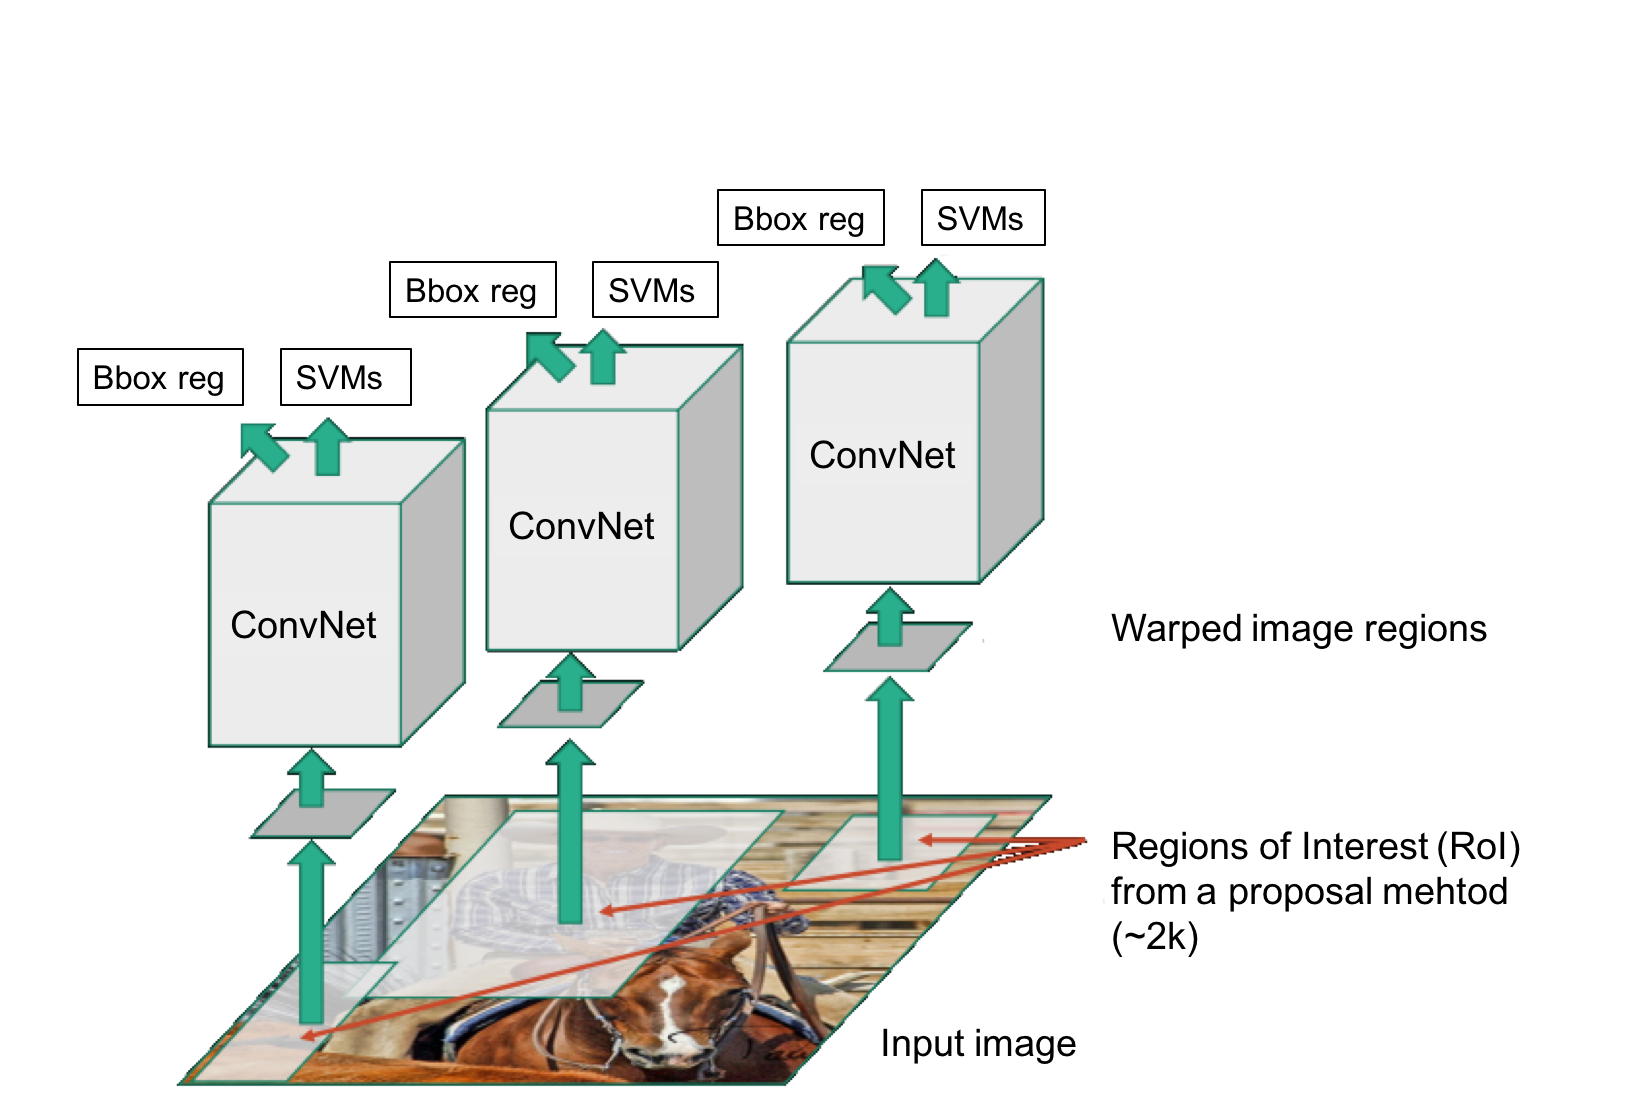
\includegraphics[width=12cm]{images/mt/rcnn.png}
	\caption{R-CNN takes external region proposals, warps the region to a uniform shape, and extracts the features separately. The extracted features are then used to classify the region, and calculate bounding box regression externally.}
	\label{fig:rcnn}
\end{figure}
\bigbreak
\subsection{Fast Region Based Convolutional Neural Network}\label{s:fastrcnn}
Fast Region based CNNs \cite{Girshick:2016:RCN:2881668.2882239} are aimed to improve the classification accuracy and feature vector extraction speed of the interest regions, generated also with selective search. An intermediate convolutional feature map is extracted from the whole input image with a fully convolutional neural network, also called as base network in \citep{journals/corr/SermanetEZMFL13}. The output is a downscaled feature map, which is fed to the so called RoI (region of interest) pooling layer. This layer crops regions from the map according to the appropriate downscaled region proposals, and executes a modified version of max pooling on each regions, which results in a convolutional map with a fixed-shape, regardless the size of the region.
\bigbreak
After the pooling, fully connected layers are used to calculate the final class probabilities and bounding box regressions for each region. The output of the bounding box regression are class specific small position and size adjustments, needed to refine the rough object locations.
\bigbreak
The proposed network is trained for K+1 classes, where K is the number of object classes, and the background is also modelled as a separate class. During training, the positive examples are chosen, regarding the intersection over union (IoU) value to the groundtruth. This value is widely used for measuring the overlapping between regions, regardless the actual size of the regions. The calculation between two regions, $R_1$ and $R_2$ is as follows:
\bigbreak
\begin{equation}
        \frac{area ( R_1 \cap R_2 )}{area ( R_1 \cup R_2 )}
        \label{eq:iou}
\end{equation}
\bigbreak
For positive training examples there are thoose regions applied, which have an IoU with the groundtruth at least 0.5. For the background class are the examples with IoU [0.1,0.5) used.
\bigbreak
The network is trained with a multi-task loss function for classification and bounding box regression, defined as:
\bigbreak
\begin{equation}\label{eq:frcnn-loss}
	L(p, u, t^u, v) = L_{cls}(p, u) + \lambda [u \ge 1] L_{loc}(t^u, v)
\end{equation}
\bigbreak
where $p$ is the computed class probabilities, $u$ is the groundtruth class, $t^u$ is the predicted bounding box offset vector for every classes, and v is the groundtruth bounding box position and size.
The probabilities are calculated with softmax as usual, so the log loss is used for the classification error: $L_{cls}(p,u) = -logp_u$. Since the bounding box regressor cannot be trained with background images, its error is not added to the complete loss. This is achieved, by setting the label of the background class to zero, and using the term $[u \ge 1]$, which is 1 if $u \ge 1$, and 0 otherwise. For regression loss, a smooth version of L1 loss is used, which is defined as follows:
\bigbreak
\begin{align}\label{eq:smoothl1loss}
	L_{loc}(t^u, v) = \sum\limits_{i \in (x, y, w, h)} smooth_{L_{1}} (t_{i}^u, v_i)\\
	smooth_{L_{1}} (x) = \begin{cases}
               0.5 x^2 & \text{if } \abs{x} < 1\\
               \abs{x}-0.5 & \text{otherwise}
            \end{cases}
\end{align}
\bigbreak
The improvements of this method compared to the previous region based CNN introduced in section \ref{s:rcnn} are as follows:
\begin{itemize}
	\item\textbf{Joint feature extraction:} much shorter training and inference time is achieved by the lower computational redundancy of running convolutional layers on the whole image only once, rather then for every proposed regions.
	\item\textbf{One network:} the feature extraction and the classification happens in the same network. This has more advantages:
	\begin{itemize}
	        \item This results again in faster test and training times, due to the unnecessity of writing the extracted feature vectors to disk, which incidentally could require e.g. hundreds of gigabytes of storage \cite{Girshick:2016:RCN:2881668.2882239} for the VOC07 trainval set \cite{pascal-voc-2007}.
	        \item As the backpropagation is implemented through the RoI pooling layer, the whole network, together with the convolutional layers, can be trained jointly, against earlier implementations, like R-CNN \cite{DBLP:journals/corr/GirshickDDM13} or spatial pyramid pooling networks (SPPnet) \cite{DBLP:journals/corr/HeZR014}.
	\end{itemize}
	\item\textbf{Minibatch from a few images:} Faster training speed is achieved by collecting a minibatch only from two images, rather than every region from different images. This method is proved to converging within similar times, despite the high correlated regions.
\end{itemize}
\bigbreak
\begin{figure}[h!]
	\centering
	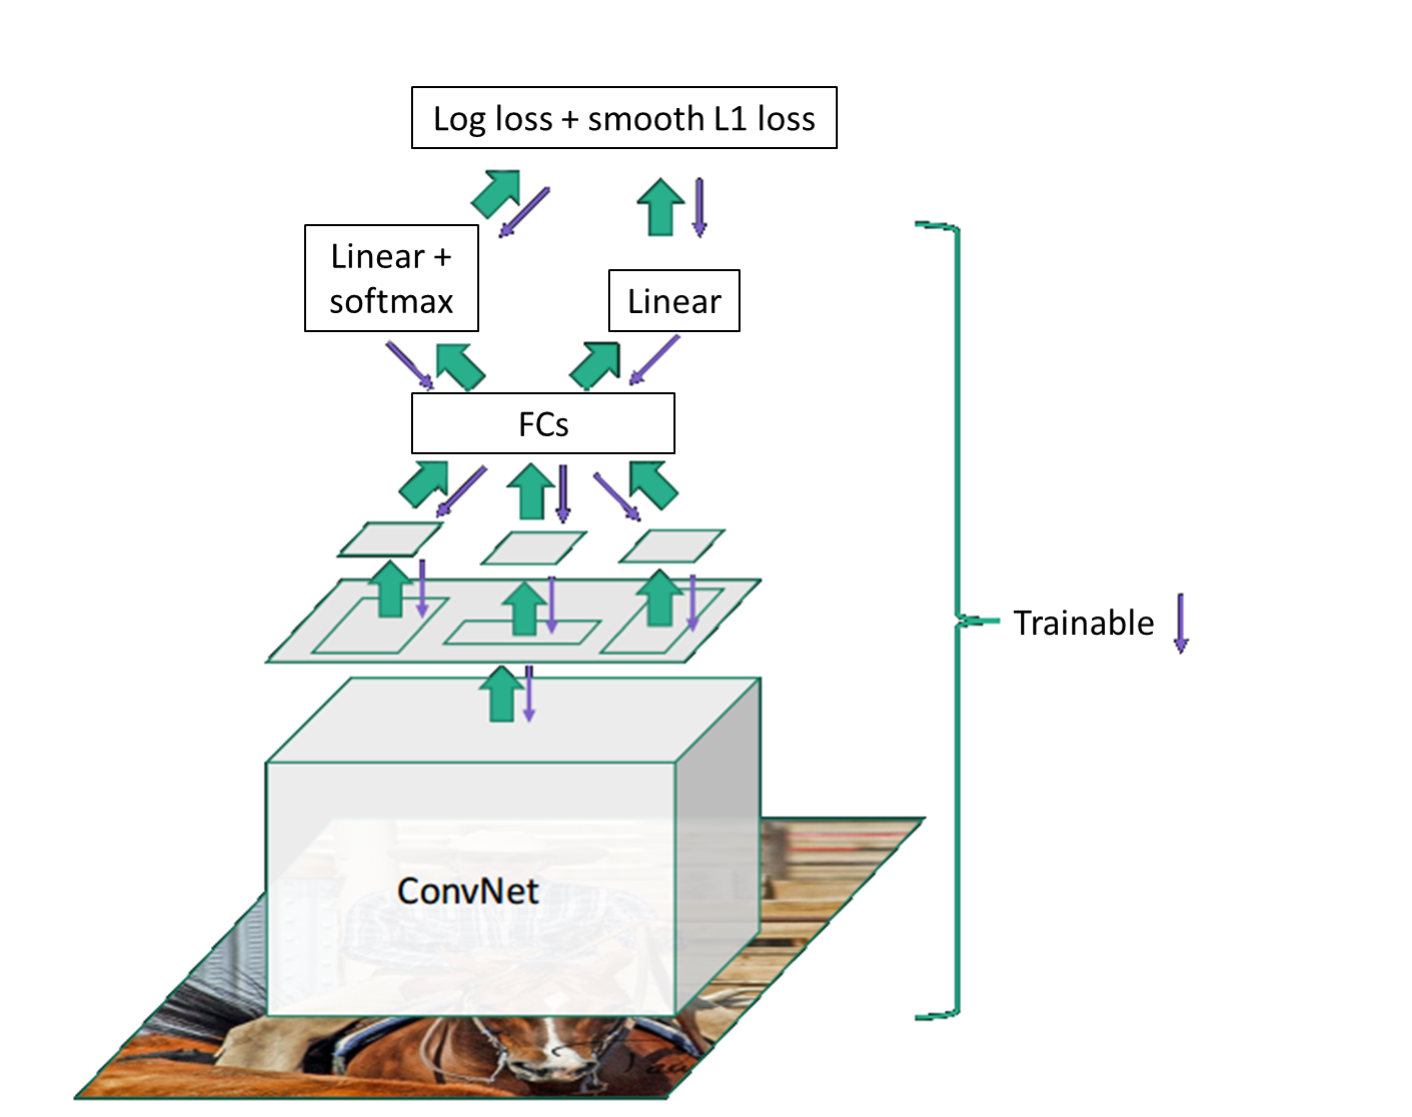
\includegraphics[width=12cm]{images/mt/fast-rcnn.png}
	\caption{Fast R-CNN uses external proposals, then infers the complete image with a fully convolutional network. The proposals is then used to crop regions from the feature map with RoI pooling. The cropped region is then classified and the region coordinates are adjusted with a fully connected network.}
	\label{fig:fastrcnn}
\end{figure}
\bigbreak
\subsection{Faster Region Based Convolutional Neural Network}\label{s:fasterrcnn}

A great disadvantage of the Fast R-CNN method is, that the region proposals are generated externally. Girshick et.at. introduces Faster R-CNN \cite{NIPS2015_5638}, which generates the interest regions within the neural network nearly cost-free (10ms pro image). This system consists of a region proposal system and a Fast R-CNN object detector.
\bigbreak
\subsubsection{Region Proposal Network}

The convolutional feature map, extracted by the base network, is processed by the RoI pooling layer. Additionally a thin fully convolutional network, the region proposal network (RPN), is also utilized on the convolutional maps, to generate the proposals. Reference boxes, called "anchors" are generated at every position of the conv feature map, in different scales and different aspect ratios. This ensures the scale invariance of the objects. A convolutional layer with 3x3 kernel extracts a fixed-size vector from every window of the conv map, where in each window 9 anchors are considered. As the fully convolutional network iterates through the conv map in a sliding window fashion, translation invariance is granted. An objectness score and bounding box offset is then calculated for every anchor, by different classifiers and regressors, specialized in a specific scale and aspect ratio.
\bigbreak
\begin{figure}[h!]
	\centering
	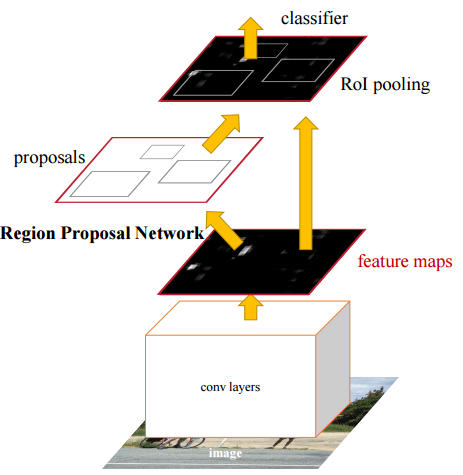
\includegraphics[width=8cm]{images/mt/faster-rcnn.png}
	\caption{Faster Region Based Convolutional Neural Network consists of a Fast R-CNN and a region proposal network (RPN). Fast R-CNN is responsible for the feature map extraction from the whole image, and classify regions from that. The RPN is an in-network implemented proposal system, for generating candidate object locations in a fast way.}
	\label{fig:faster-rcnn}
\end{figure}
\bigbreak
\subsubsection{Training}
As the RPN is a class agnostic object detector, it should detect all the types of objects, which the network is trained on. For this purpose, the class informations, during training of RPN, can be discarded. Positive examples are collected from the proposals with an IoU higher than 0.7 with any groundtruth. Negative label is assigned for regions, which have an IoU, lower than 0.3.
\bigbreak
Since the objective of the RPN is the same as for Fast R-CNN, namely to classify regions and regress bounding box coordinates, the loss functions for training the RPN can the same multi-task loss, which are used for training a Fast R-CNN, detailed in section \ref{s:fastrcnn}.
\bigbreak
Earlier versions of the system suggested to train the complete system in an alternating way. First the RPN will be trained with a CNN, pretrained on e.g. the ImageNet dataset \cite{imagenet_cvpr09}. The trained RPN will then be used to propose regions, and train the Fast R-CNN part with them. The CNN of the fine-tuned Fast R-CNN is then used to train the RPN again, and this process is repeated iteratively. Later, it has been proven, that training the whole network of the faster R-CNN can be performed in an end to end manner, with marginal performance drop. This means, that all the parts of the system can be trained jointly.